\section{Experiments}
\label{sec:experiments}
% Description of your testbed;
% List of questions your experiments are designed to answer.
% Details of the experiments; observations.

In this section, we first present the dataset we use in our experiments as well
as the parameters for each model. Note that we fine tuned these parameters to
achieve the best possible outcomes before we add our modification to the code.
Next, we present the results and conclude findings we get from our experiments,
including those negative results and the lessons learned in this project.

\subsection{Dataset and Implementation Parameters}
We experiment on three datasets---a hand-written digit dataset (MNIST),
two tiny images datasets (CIFAR-10 and CIFAR-100).
Specifications of datasets are summarized in Table~\ref{datasets}.
\vspace{-7pt}
\begin{table}[!htbp]
\centering
\begin{tabular}{| c | c | c | c | c |}
\hline
Dataset & Description & Class & Training Set Size & Testing Set Size \\
\hline
MNIST & hand-written digits & 10 & 60,000 & 10,000\\
CIFAR-10 & 32x32 RGB images & 10 & 50,000 & 10,000\\
CIFAR-100 & 32x32 RGB images & 100 & 50,000 & 10,000\\
\hline
\end{tabular}
\caption{Datasets: MNIST, CIFAR-10, CIFAR-100}
\label{datasets}
\end{table}

We preprocess CIFAR-10 and CIFAR-100 by grey-scaling every image using the following formula:
\[
Y = 0.2126 * R + 0.7152 * G + 0.0722 * B
\]
In other words, every pixel in the image is now a linear combination of its
original RGB values. These two datasets are preprocessed due to technical
implementation limitations (which will be fixed after the deadline), not
machine learning theory reasons.

Our neural network models are implemented using Python Theono Library. The
starter code is from DeepLearning.net. Parameters of each neural
network models are summarized in Table~\ref{params}.
\vspace{-7pt}
\begin{table}[!htbp]
\centering
\begin{tabular}{| c | c |}
\hline
Model & Parameters \\
\hline
Logistic Regression (LR) & learning rate = 0.13 \\
Multi-layer Logistic Regression (MLP) & LR + hidden units = 500 \\
Convolutional Neural Network & MLP + window size = 5x5, downsample = 2x2\\
\hline
\end{tabular}
\caption{Parameters of Neural Network Models}
\label{params}
\end{table}

We use stochastic logistic regression with learning rate = 0.13.
In Multi-layer Logistic Regression, there are 500 neurons in the hidden
layer. During feature mapping of Convolutional Neural Network, windows
are of size 5 by 5 and downsample is of size 2 by 2.

In our experiments, different models may run different number of
iterations. This is because we set a threshold of accuracy increase when
training the model. If the model's accuracy increase is less than the
threshold, we stop training the model. Hence some models run more
iterations as long as their accuracy increases are above the threshold.

\subsection{Adding Noise into Logistic Regression}
Figure~\ref{logistic} shows test error rate using noise-free and
noise-added Logistic Regression on MNIST.
\begin{figure}[!htbp]
\centering
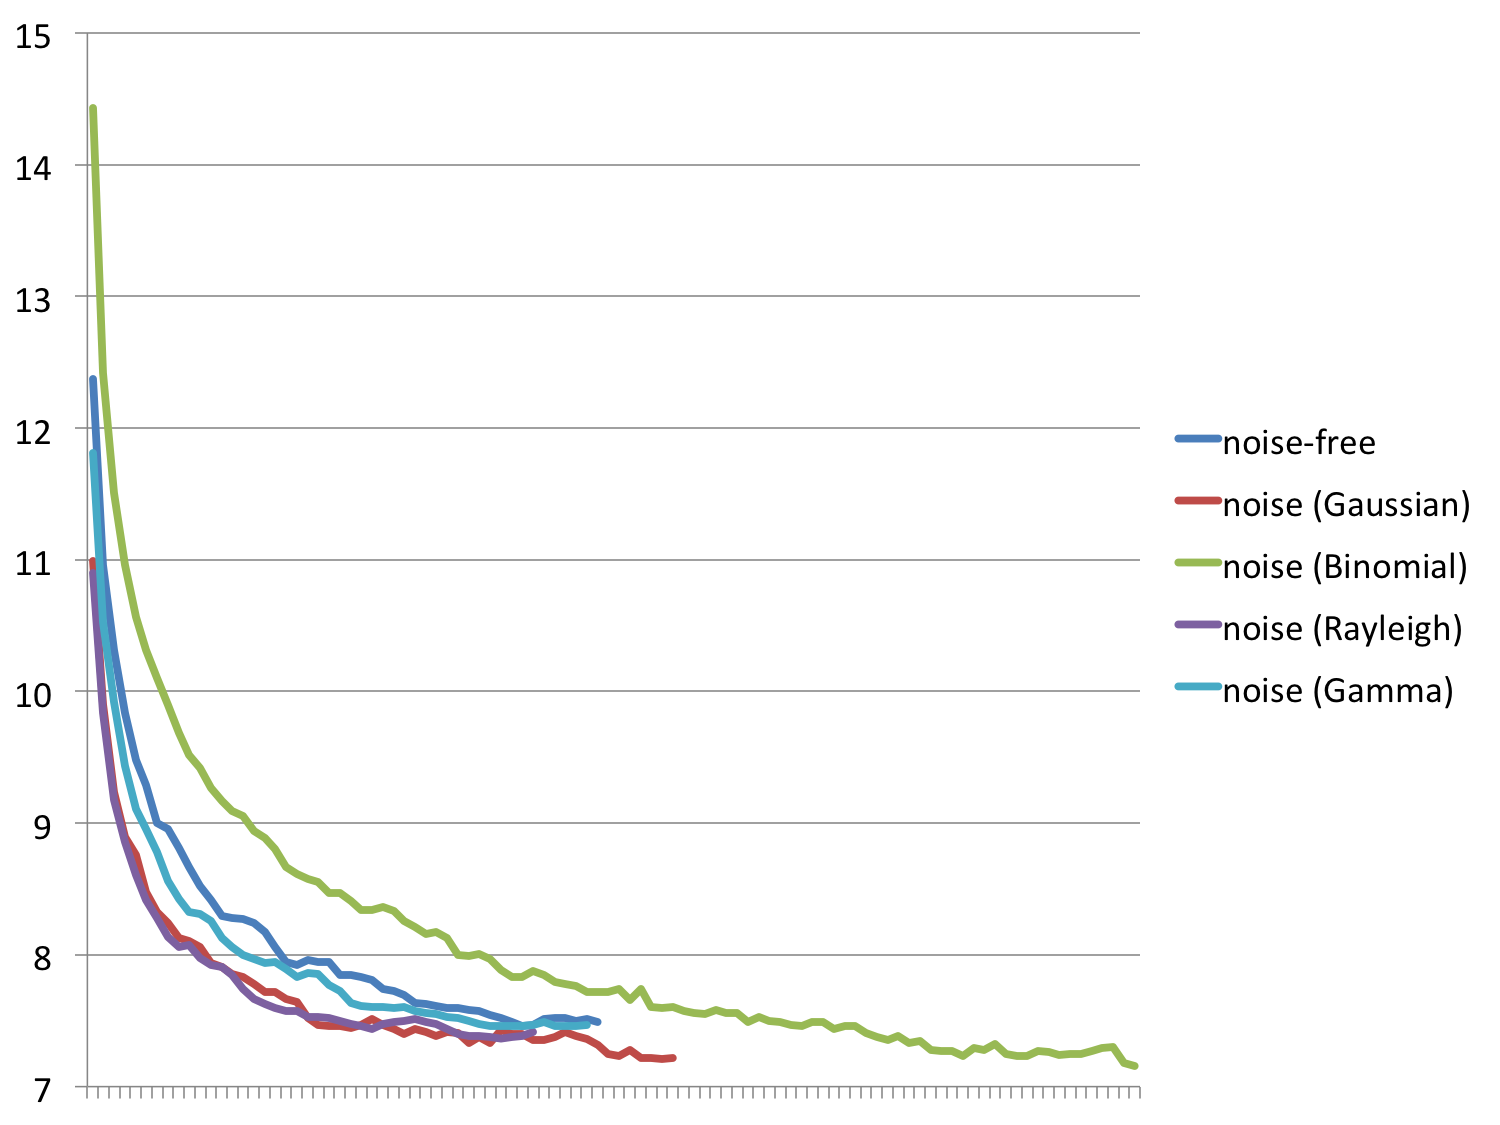
\includegraphics[width=215pt]{f-figs/logistic.png}
\caption{Logistic Regression with Noise on MNIST}
\label{logistic}
\end{figure}

In Figure~\ref{logistic}, the vertical axis is test error rate (\%), the
horizontal axis is number of iterations. The experiments all run on MNIST.
The noise-free line shows test error rate using a noise-free Logistic
Regression model.
The noise(Gaussian) line shows test error rate when $\mask_{Gau}$ is applied during gradient descent.
The noise(Binomial) line shows test error rate when a mask generated from
$Bin(1,0.5)$ is applied during gradient descent.
The noise(Rayleigh) line shows test error rate when a mask generated from
$Rayleigh(1)$ is applied during gradient descent.
The noise(Gamma) line shows test error rate when a mask generated from
$Gamma(1,1)$ is applied during gradient descent.

{\bf Finding 1: {\em A reasonable amount, and a reasonable amplitude of noise
improves deep neural network model's accuracy, while a noise that is too
significant does not.}} \\
As showed in Figure~\ref{logistic}, {\em noise-added models achieve better
accuracy compared to the noise-free model.}
Noise(Binomial) model has the lowest test error rate (7.156\%) among the
five experiments. However, it also has the lowest convergence rate.
This is a phenomenon we have observed throughout the project.
{\em Though adding noise can improve accuracy, the side effect is that it
will take longer to train the model, hence decrease convergence rate.}

\subsection{Adding Noise into Multi-layer Logistic Regression}
Figure~\ref{mlp} shows test error rate using noise-free and noise-added
Multi-layer Logistic Regression on MNIST.
\begin{figure}[!htbp]
\centering
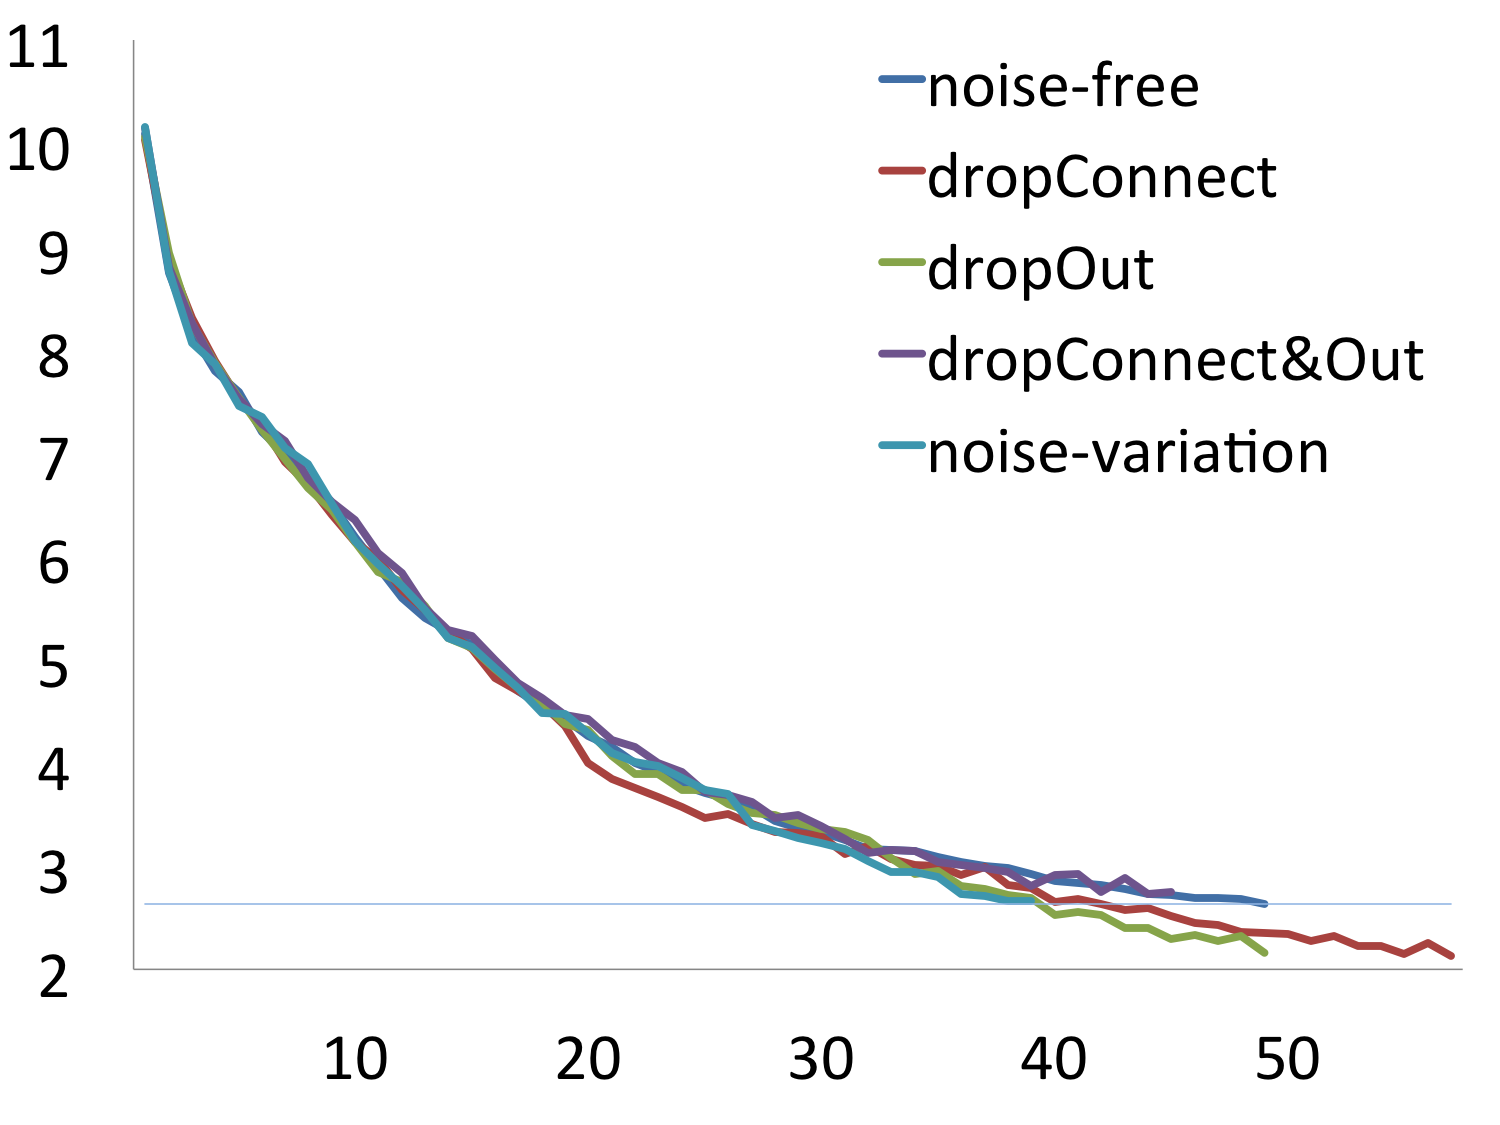
\includegraphics[width=215pt]{f-figs/mlp.png}
\caption{Multi-layer Logistic Regression with Noise on MNIST}
\label{mlp}
\end{figure}

In Figure~\ref{mlp}, the vertical axis is test error rate (\%), the
horizontal axis is number of iterations. The experiments all run on MNIST.
The noise-free line shows test error rate using a noise-free Multi-layer
Logistic Regression.
The dropConnect line shows test error rate when a mask generated from
$Bin(1,0.99)$ is applied to $W_{input}$.
The dropOut line shows test error rate when a mask generated from
$Bin(1,0.99)$ is applied to $W_{output}$.
The dropConnect\&Out line shows test error rate when mask generated
from $Bin(1,0.99)$ is applied to both $W_{input}$ and $W_{output}$.
The noise-variation line shows test error rate when a mask generated from
Gaussian $\mathcal{N}(0,0.01)$ is added to $W_{input}$.

{\bf Finding 2: {\em Deep learning models with noise perform no worse than
the noise-free model.}} \\
As showed in Figure~\ref{mlp}, {\em noise-added models perform no worse than the noise-free model.}
Since the test error rate of the noise-free model is already
quite low (2.63\%), it is difficult for noise-added models to significantly
improve accuracy. We notice that dropOut model and dropConnect model
perform better than dropConnect\&Out model and noise-variation model.
It is difficult to provide a conclusive explanation for this observation at
the moment because we have not finished fine-tuning our noise-added models.
{\em It is possible that noise from certain distributions is more
likely to prevent overfitting and hence improve accuracy.}

Figure~\ref{mlp10} shows test error rate using noise-free and noise-added
Multi-layer Logistic Regression on CIFAR-10.
\begin{figure}
\centering
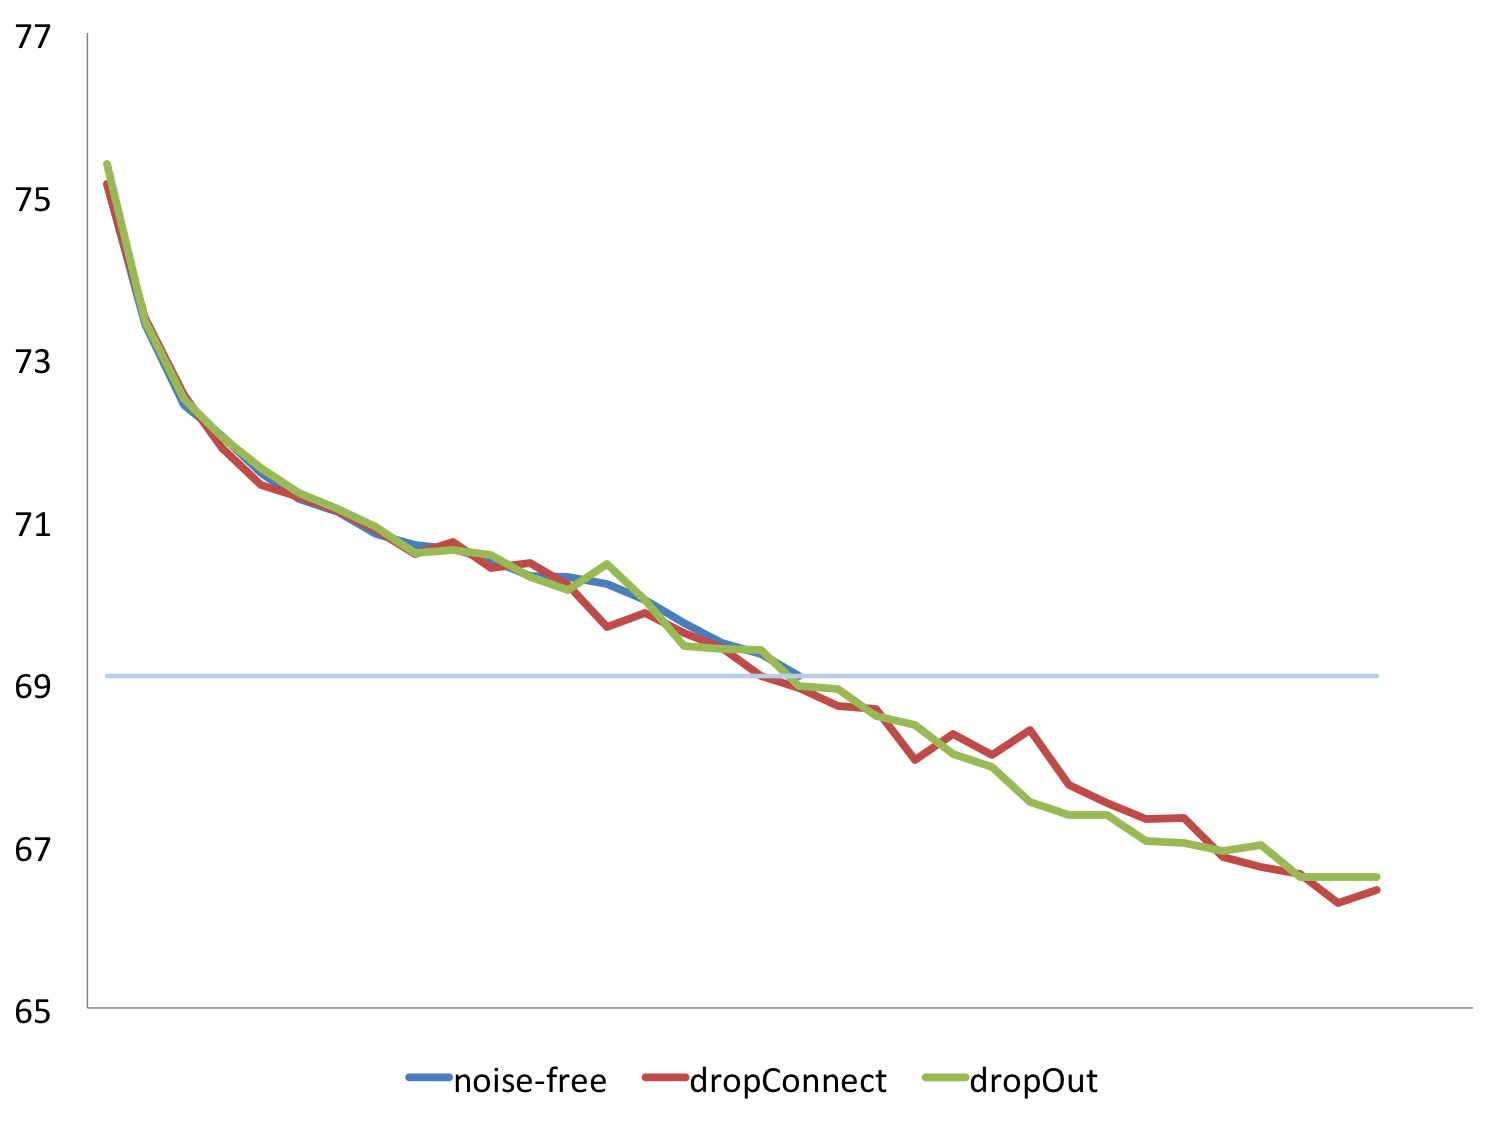
\includegraphics[width=215pt]{f-figs/mlp10.png}
\caption{Multi-layer Logistic Regression with Noise on CIFAR-10}
\label{mlp10}
\end{figure}
In Figure~\ref{mlp10}, the vertical axis is test error rate (\%), the
horizontal axis is number of iterations. The experiments all run on
CIFAR-10. The noise-free line, dropConnect line and dropOut line use
the same models as experiments in Figure~\ref{mlp}, respectively.

{\bf Finding 3: {\em Deep learning models with noise can take more iterations to
converge as the test error fluctuates due to noise.}} \\
As showed in Figure~\ref{mlp10}, noise-added models perform much better than
noise-free model, though it takes longer to train noise-added models.
An interesting observation is that {\em as training iterations increase,
test error rate of noise-added models fluctuates.} This is another side
effect of adding noise into the model.

{\bf Finding 4: {\em Noise added to earlier stage of the deep learning models
can be better integrated and generate less fluctuation.}} \\
From the above experiments using MLP, we observe that models with noise added
between input layer and hidden layer outperform other noise-added models.
An intuitive explanation for this phenomenon is that {\em noise added to
earlier stage of the model can be better integrated} while noise added to
later stage of the model tends to cause more fluctuation.

\subsection{Adding Noise into Convolutional Neural Network}
Figure~\ref{convo} shows test error rate using noise-free and noise-added
Convolutional Multi-layer Logistic Regression on MNIST.
\begin{figure}[!htbp]
\centering
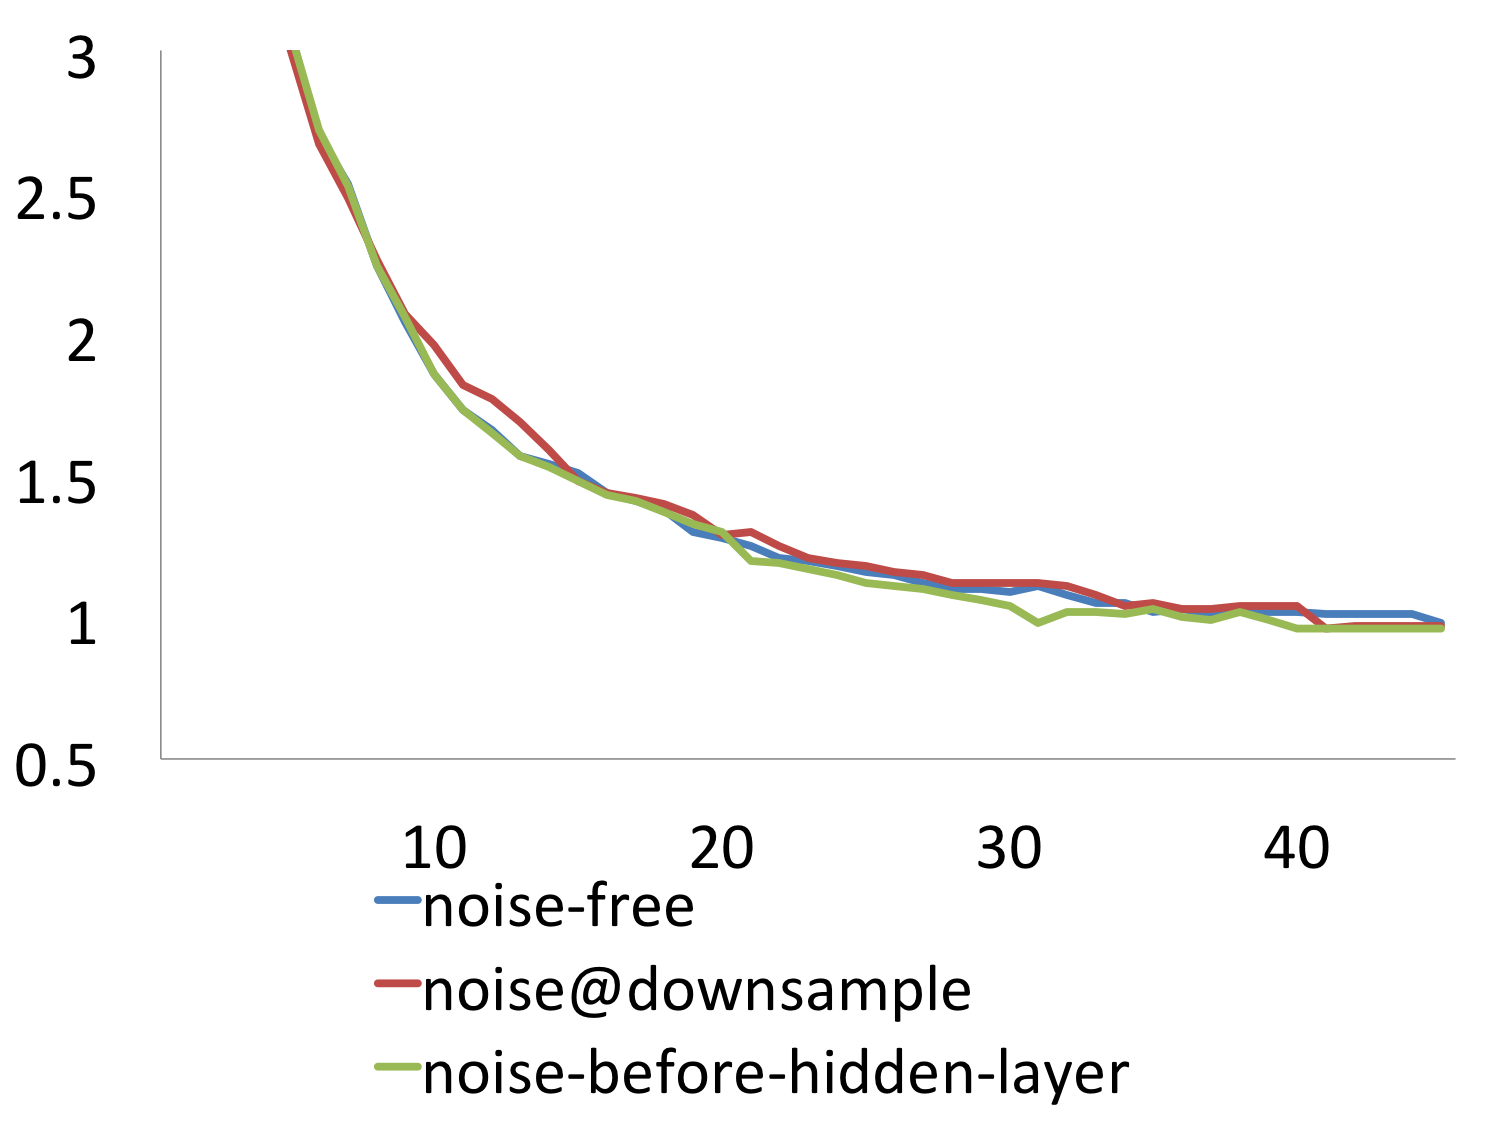
\includegraphics[width=215pt]{f-figs/convo.png}
\caption{Convolutional Neural Network with Noise on MNIST}
\label{convo}
\end{figure}
In Figure~\ref{convo}, the vertical axis is test error rate (\%), the
horizontal axis is number of iterations. The experiments all run on MNIST.
The noise-free line shows test error rate when using a noise-free
Convolutional Neural Network. The noise@downsampe line shows test error
rate when noise is added during downsample process. The noise-before-hidden-layer line shows test error rate when noise is added right before hidden layer.

{\bf Finding 5: {\em The convergence rate is faster for deep learning models
with noise.}} \\
As showed in Figure~\ref{convo}, the three models perform equally well.
We observe that as the number of iterations increases, {\em noise-added
models converge slightly faster}. This phenomenon is interesting because it is unexpected.
Similarly phenomenon appears in Figure~\ref{convo10} as well.

Figure~\ref{convo10} shows test error rate using noise-free and noise-added
Convolutional Multi-layer Logistic Regression on CIFAR-10.
\begin{figure}[!htbp]
\centering
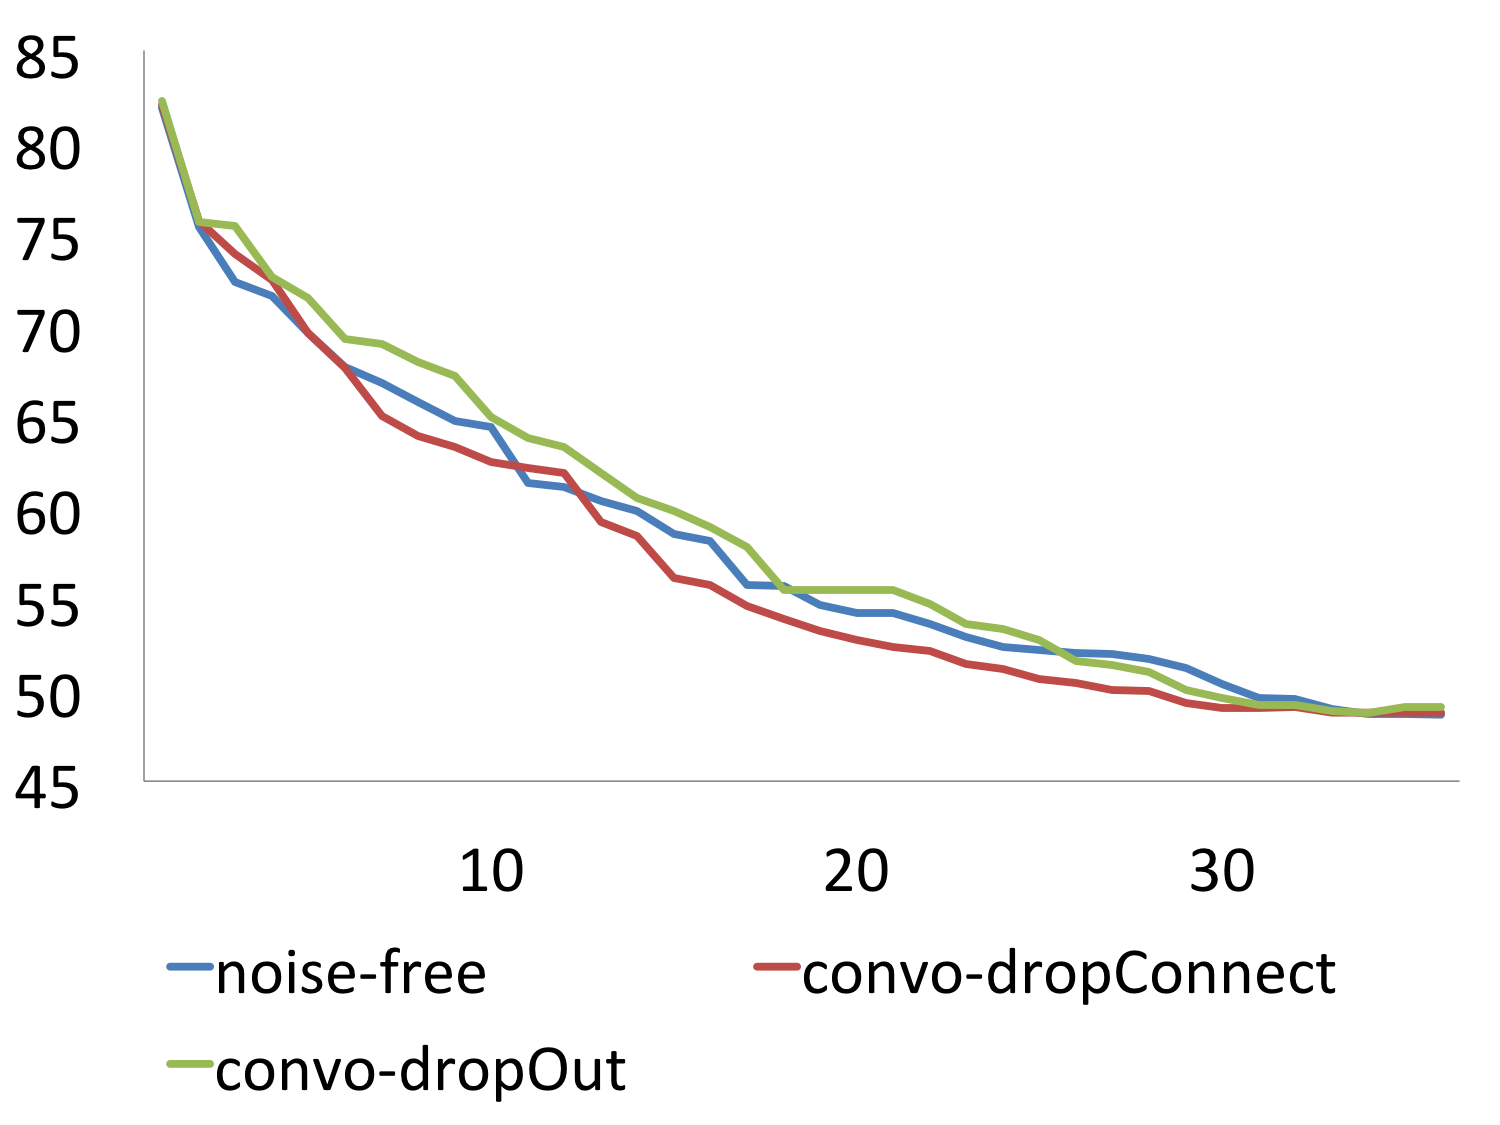
\includegraphics[width=215pt]{f-figs/convo10.png}
\caption{Convolutional Neural Network with Noise on CIFAR-10}
\label{convo10}
\end{figure}
In Figure~\ref{convo10}, the vertical axis is test error rate (\%), the
horizontal axis is number of iterations. The experiments all run on
CIFAR-10. The noise-free line shows test error rate when using a
noise-free Convolutional Neural Network.
The convo-dropConnect line shows test error rate when the MLP part of the
model has noise added between input layer and hidden layer.
The convo-dropOut line shows test error rate when the MLP part of the model
has noise added between hidden layer and output layer.

{\bf Finding 6: {\em Noise improves both accuracy and convergence rate more with
complex deep learning models.}} \\
As showed in Figure~\ref{convo10}, the three models achieve the same lowest
test error rate. However, through the training process, {\em the
noise-added model (convo-dropConnect) converges faster than the noise-free
model}. The intuition behind this phenomenon is that since Convolutional
Neural Network is a complicated model, noise is better integrated and
absorbed. We conjecture that {\em noise added to complicated deep
learning models can improve not only accuracy but also convergence rate}.

\subsection{Negative Results}

{\bf Lesson Learned: {\em Complex deep learning models can integrate noise
better than simple models.}}
Figure~\ref{neg} shows some negative results from our experiments.
We experiment noise-free and noise-added Logistic Regression on CIFAR-100.
The noise-added model perform much worse than noise-free model. The
explanation for this result is that Logistic Regression model is too
simple to integrate noise when running CIFAR-100. This agrees with our
previous conjecture that {\em complicated models are better at integrating
noise}.
\begin{figure}[!htbp]
\centering
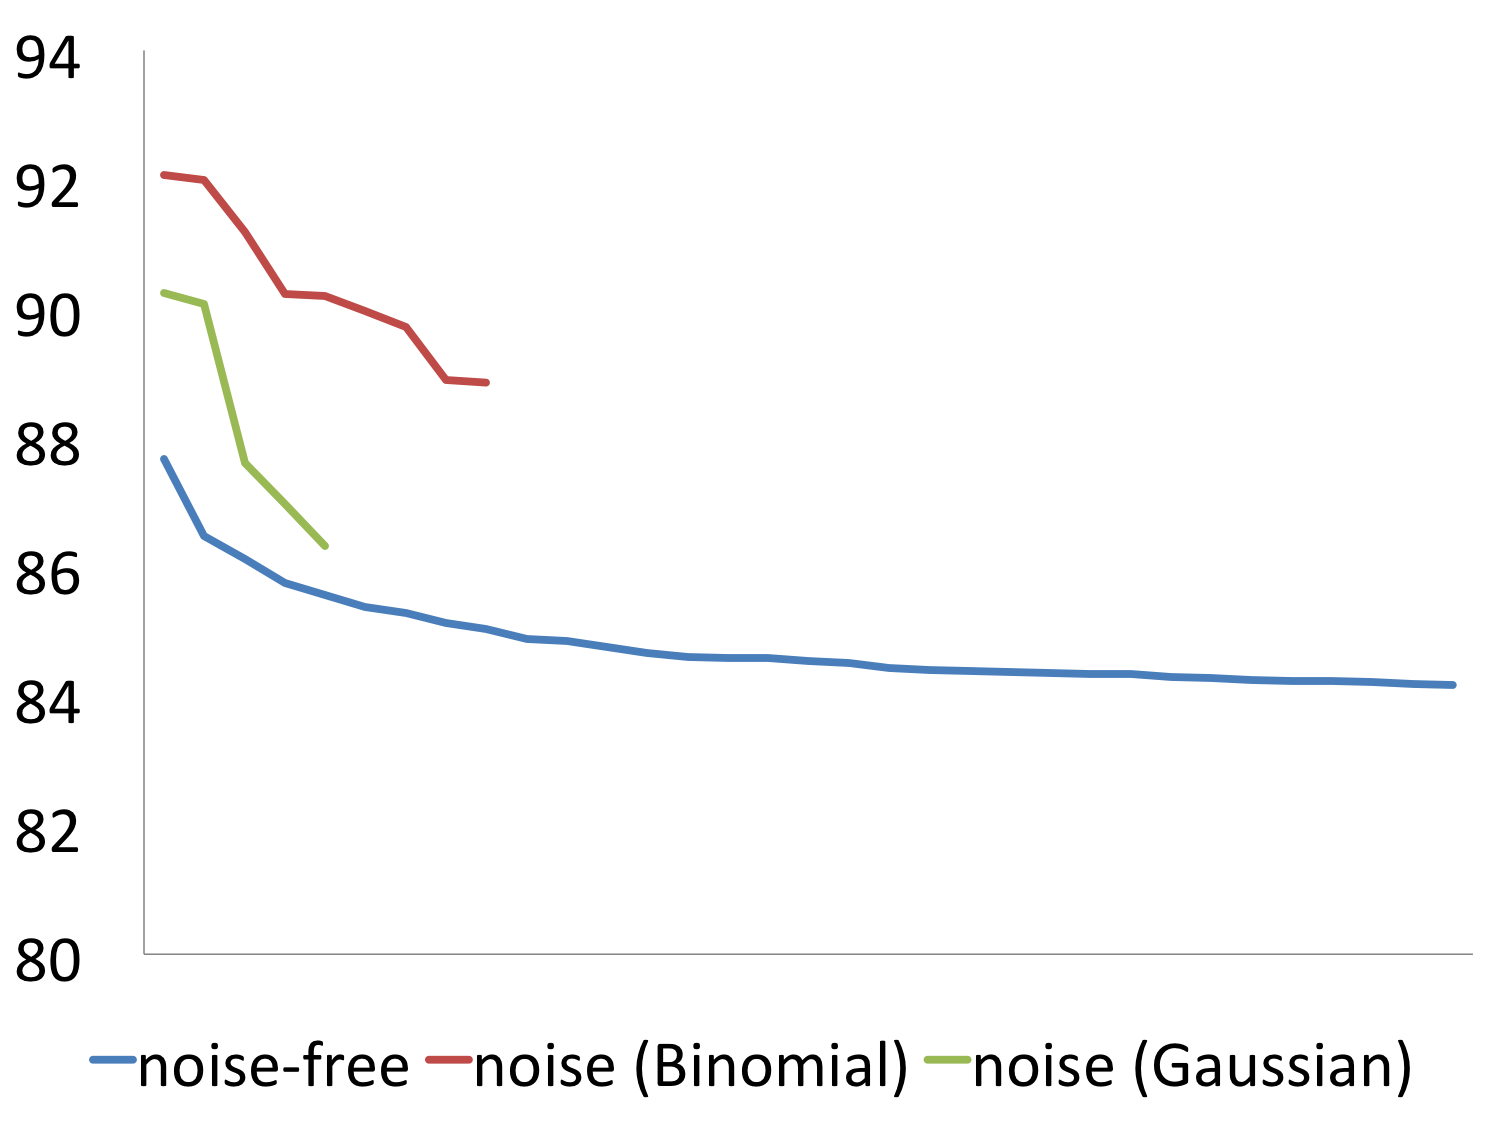
\includegraphics[width=215pt]{f-figs/neg.png}
\caption{Negative Results on CIFAR-100}
\label{neg}
\end{figure}
